\begin{frame}
  \section{Divergens og curl}
  \frametitle{Divergens}

\begin{itemize}
  \item Et vektorfelt kan betraktes som bevegelse av væsker eller gasser
  \item Divergens er \emph{endring} i fluks. Altså en operator som tar inn et vektorfelt, og gir ut en
    skalar som viser hvor mye væsketettheten endrer seg i ett punkt.
  \item Formelen for divergens er
    %
    \begin{equation*}
      \div \F = \nabla \cdot \F
              = \diffp{{F_1}}{x} + 
              \diffp{{F_2}}{y} +
              \cdots 
    \end{equation*}
    %
    Hvor $\F = (F_1, F_2, \ldots, F_n)$ er komponentene til $\F \colon \R^m \to \R^n$.
\end{itemize}

\begin{figure}
  \centering
  \begin{minipage}{.30\textwidth}
    \centering
  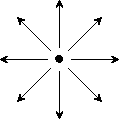
\includegraphics[scale=1.5]{../img/div-positive}
  \caption{$\nabla \cdot \F > 0 $}
\end{minipage}\hfill
\begin{minipage}{.30\textwidth}
    \centering
  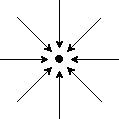
\includegraphics[scale=1.5]{../img/div-negative}
  \caption{$\nabla \cdot \F <0 $}
\end{minipage}
\begin{minipage}{.30\textwidth}
    \centering
  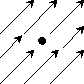
\includegraphics[scale=1.5]{../img/div-null}
  \caption{$\nabla \cdot \F = 0$}
\end{minipage}
\end{figure}
\end{frame}

\begin{frame}
  \frametitle{Curl}
  \begin{itemize}
  \item Curlen viser hvor mye og i hvilken retning et
      vektorfelt “roterer”.
      \item Curlen er en vektor som peker i rotasjonsaksen og er proposjonal med rotasjonshastigheten.
    \item Dersom vektorfeltet roterer mot klokken sier vi at kurlen er positiv,
mot klokken er den negativ, mens dersom vektorfeltet er rotasjonsfritt er kurlen
      null.
    \item $\curl \F = \nabla \times \F =
      \begin{vmatrix} \I & \J & \K \\ \frac{\partial}{\partial x} &
        \frac{\partial}{\partial y} & \frac{\partial}{\partial z}\\ F_1 & F_2  & F_3
      \end{vmatrix} \ $ og $ \ \2d-curl \F = \diffp{{F_2}}{x} - \diffp{{F_1}}{y} $.
  \end{itemize}
  \begin{center}
      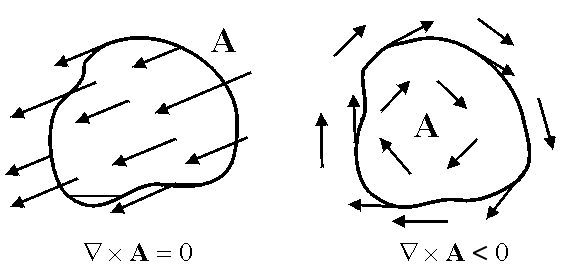
\includegraphics[scale=0.5]{../img/curl-negative.png}
\end{center}
\end{frame}

\begin{frame}
  \frametitle{Curl}
  \begin{figure}
  \centering
  \begin{minipage}{.30\textwidth}
    \centering
  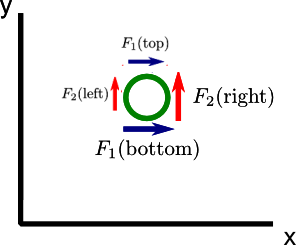
\includegraphics[scale=0.75]{../img/rotation-2}
\end{minipage}
\begin{minipage}{.30\textwidth}
  \onslide<2->{%
  \begin{equation*}
    \phantom{1} \hspace{2cm} \2d-curl \F = \diffp{{F_2}}{x} - \diffp{{F_1}}{y}
  \end{equation*}}
\end{minipage}\hspace{2cm}
\end{figure}
\onslide<3->{
  \begin{align*}
    \label{eq:curl}
    \curl \F & = \nabla \times \F \\
    & = \left( \diffp{{F_3}}{y} - \diffp{{F_2}}{z} \right) \I
    + \left( \diffp{{F_1}}{z} - \diffp{{F_3}}{x} \right) \J
    + \left( \diffp{{F_2}}{x} - \diffp{{F_1}}{y} \right) \K.
  \end{align*}%
}
\end{frame}

\begin{frame}
  \begin{oppgave}{V2013, Oppgave 4}
    Vis sier at en funksjon er $C^2$ om alle andreordens partiellderiverte er
    kontinuerlige. Vis at om $f$ er en $C^2$ funksjon, så er $\curl\bigl( \nabla
    f\bigr) = \vek{0}$. Si klart fra hvordan du bruker at funksjonen er $C^2$. 
  \end{oppgave}
  \only<1>{%
  \begin{equation*}
    \curl \F =
    \begin{vmatrix}
      \I & \J & \K \\
      \frac{\partial}{\partial x} & \frac{\partial}{\partial y} & \frac{\partial}{\partial z}\\
      F_1 & F_2  & F_3
    \end{vmatrix}
     \qquad \text{og} \qquad
     \nabla f = \left( \diffp{f}{x}, \diffp{f}{y}, \diffp{f}{z} \right)
   \end{equation*}} \only<2->{%
 \begin{align*}
   \curl \bigl( \nabla f \bigr)
   \only<1-6>{& =
     \begin{vmatrix} \only<2>{\I} \only<3>{\circled{\I}} \only<6->{\I}
       & \only<2>{\J} \only<4>{\circled{\J}} \only<6->{\J}
       & \only<2>{\K} \only<5>{\circled{\K}} \only<6->{\K} \\
         \only<2>{\frac{\partial}{\partial x}} \only<4->{\frac{\partial}{\partial x}}
       & \only<2-3>{\frac{\partial}{\partial y}} \only<5->{\frac{\partial}{\partial y}}
       & \only<2-4>{\frac{\partial}{\partial y}} \only<6->{\frac{\partial}{\partial y}}\\
         \only<2>{\frac{\partial f}{\partial x}} \only<4->{\frac{\partial f}{\partial x}}
       & \only<2-3>{\frac{\partial f}{\partial y}} \only<5->{\frac{\partial f}{\partial y}}
       & \only<2-4>{\frac{\partial f}{\partial z}} \only<6->{\frac{\partial f}{\partial z}}
    \end{vmatrix}}
        \only<7>{&}\only<3-7>{=\I \begin{vmatrix} \frac{\partial}{\partial y} & \frac{\partial f}{\partial z} \\
                  \frac{\partial}{\partial z} & \frac{\partial f}{\partial y} \end{vmatrix}}
        \only<4-7>{- \J \begin{vmatrix} \frac{\partial}{\partial x} & \frac{\partial f}{\partial z} \\
                  \frac{\partial}{\partial x} & \frac{\partial f}{\partial y} \end{vmatrix}}
        \only<5-7>{+ \K \begin{vmatrix} \tfrac{\partial}{\partial y} & \tfrac{\partial f}{\partial x} \\
            \tfrac{\partial}{\partial z} & \tfrac{\partial f}{\partial y} \end{vmatrix}\\}
   \only<7->{
    & = \I \left( \tfrac{\partial}{\partial y} \tfrac{\partial f}{\partial z}
      -           \tfrac{\partial}{\partial z} \tfrac{\partial f}{\partial y} \right)
      - \J \left( \tfrac{\partial}{\partial y} \tfrac{\partial f}{\partial z}
      -           \tfrac{\partial}{\partial z} \tfrac{\partial f}{\partial y} \right)
      + \K \left( \tfrac{\partial}{\partial y} \tfrac{\partial f}{\partial z}
      -           \tfrac{\partial}{\partial z} \tfrac{\partial f}{\partial y} \right)\\}
   \only<8->{
    & = \I \left( \tfrac{\partial^2f}{\partial y \partial z} - \tfrac{\partial^2f}{\partial z\partial y} \right)
      - \J \left( \tfrac{\partial^2f}{\partial y \partial z} - \tfrac{\partial^2f}{\partial z\partial y} \right)
      + \K \left( \tfrac{\partial^2f}{\partial y \partial z} - \tfrac{\partial^2f}{\partial z\partial y} \right)}
   \only<9->{ \intertext{Siden funksjonen er $C^2$ er alle de kryss-partiellderiverte like slik at}
    & = \I 0 - \J 0 + \K 0 = \vek{0}}
  \end{align*}
}
\end{frame}





%%% Local Variables:
%%% mode: latex
%%% TeX-master: "main"
%%% End:
